\section{Introduction}\label{introduction}

Technological advances have transformed how museums document, present and interpret their collections. Immersive experiences are afforded through tools such as laser scanning, 3D printing, and virtual reality \cite{allard2005use,Wachowiak01082009,RCM_2024_3D,Kuzminsky_LaserScan_2012,Schaich_3D_2007}. These technologies form a kind of experiential authenticity, enabling encounters that evoke the past's sensory, emotional, and intellectual essence \cite{trant_Auth_1999}. However, as Pine and Gilmore note \cite{pinegilmore_2007}, achieving authenticity requires museums to navigate the delicate balance between preservation and meaningful engagement—a challenge that is particularly evident in the case of historical musical instrument collections \cite{McAlpine2014}.

Musical instruments represent a peculiar fusion of form, function, and history. Their cultural value extends beyond their visual appeal to include the tactile and auditory dimensions of use \cite{Fritz2017}. Yet, preservation concerns often limit direct interaction, reducing these artefacts to static displays. This ``red velvet cord'' approach, as theorised by McAlpine \cite{McAlpine2014}, protects fragile mechanisms but diminishes the instruments’ functional identity, disconnecting visitors from the full richness of their historical and cultural context.

The Tagliavini Collection in Bologna \cite{Tagliavini2007}, renowned for its historical keyboard instruments, exemplifies this dilemma. To address it, this project introduces an augmented replica of a historical harpsichord keyboard. 
% The project builds on an existing design borrowed from \cite{McPherson2013} and aligns with principles outlined in \cite{Masu_NIME_2023}, emphasising the importance of extending the lifecycle of existing NIMEs. 
% The project fosters and complements the augmented piano keyboard design presented by McPherson \cite{McPherson2013} and ensures the relevance of previous NIME designs beyond their original context \cite{Masu_NIME_2023}. 


The article is organised as follows: TBC



\section{Related Work and Motivations}\label{related-work}


Museums often face significant challenges in engaging visitors due to limitations in staffing and funding, which restrict how visitors can interact with collections \cite{Templeton2018, McAlpine2014}. For musical instrument museums, these challenges are compounded by the difficulty of preserving historical instruments in a playable condition \cite{McAlpine2014}. The instruments' inherent fragility and gradual decay inevitably result in a point where they can no longer be played, even when collections adhere to the strictest conservation protocols \cite{NYT_strad}. A significant cultural change has taken place in recent decades, shifting the focus from the playability of the originals to their conservation. Karp \cite{Karp1979,Karp1985} advocates for a deeper understanding of musical instruments so that enough knowledge is generated to make them as ``copyable'' as possible.

McAlpine discusses a case similar to the Tagliavini collection in his examination of the Benton Fletcher Collection at National Trust Fenton House \cite{McAlpine2014}. When these instruments were donated, Benton Fletcher stipulated that they remain playable and should continue to be maintained for tuition and public performance. A large sampling campaign was conducted, and a custom MIDI interface was designed to fulfil this requirement while preserving the original instruments' integrity. The MIDI controller, comprising two commercially available keyboards mimicking the two-manual harpsichord layout, was used by visitors to trigger the instrument samples recorded with tailored strategies for each. However, user tests identified a limitation: the commercially available weighted keys failed to provide an authentic sense of interacting with a historical keyboard \cite{McAlpine2014}. 

On the other hand, the ``Tromba Moderna'' project \cite{Baldwin2016}, a previous NIME initiative, approached the issue of musical heritage playability by recreating and augmenting a replica of a historical tromba marina. A piezo transducer was connected to a sound synthesis engine and a driver within the instrument to simulate the expected vibrations of a historical tromba marina. 

This work inherits the same philosophy as the Tromba Moderna project. By augmenting a replica of a historical harpsichord keyboard using minimally invasive electronics and controlling a MIDI-triggered sample library, the project intends to offer a tool enhancing the fruition of the Tagliavini collection whilst retaining a form of continuity with historical instrument-building traditions. Furthermore, the electronics design borrows ideas from a previous NIME by McPherson \cite{McPherson2013}. As such, the interface proposed here is not, strictly speaking, a \emph{new} musical interface, particularly in its haptic response designed to adhere to longstanding harpsichord building traditions. However, this work complements and follows up on previous reflections within the NIME community, emphasising the \emph{O} in NIME \cite{Masu_NIME_2023}. 
The intended use of the keyboard through meaningful interaction with a museum exhibit is where the novelty of this work lies, rather than solely in its technological development. Furthermore, relying on previous NIMEs, this project extends the longevity of the results beyond the scope envisaged in the original papers and enables a form of sustainability. 

Besides enhancing the visitor experience, future design iterations will serve as a research tool to explore the unique characteristics of the harpsichord and its impact on performance through the \anon{ERC-funded NEMUS} project, aiming to virtually reproduce the sound of historical keyboard instruments, and upcoming projects such as Rem@ke \cite{remake1}.

\section{Design Principles}\label{design}

\begin{figure*}
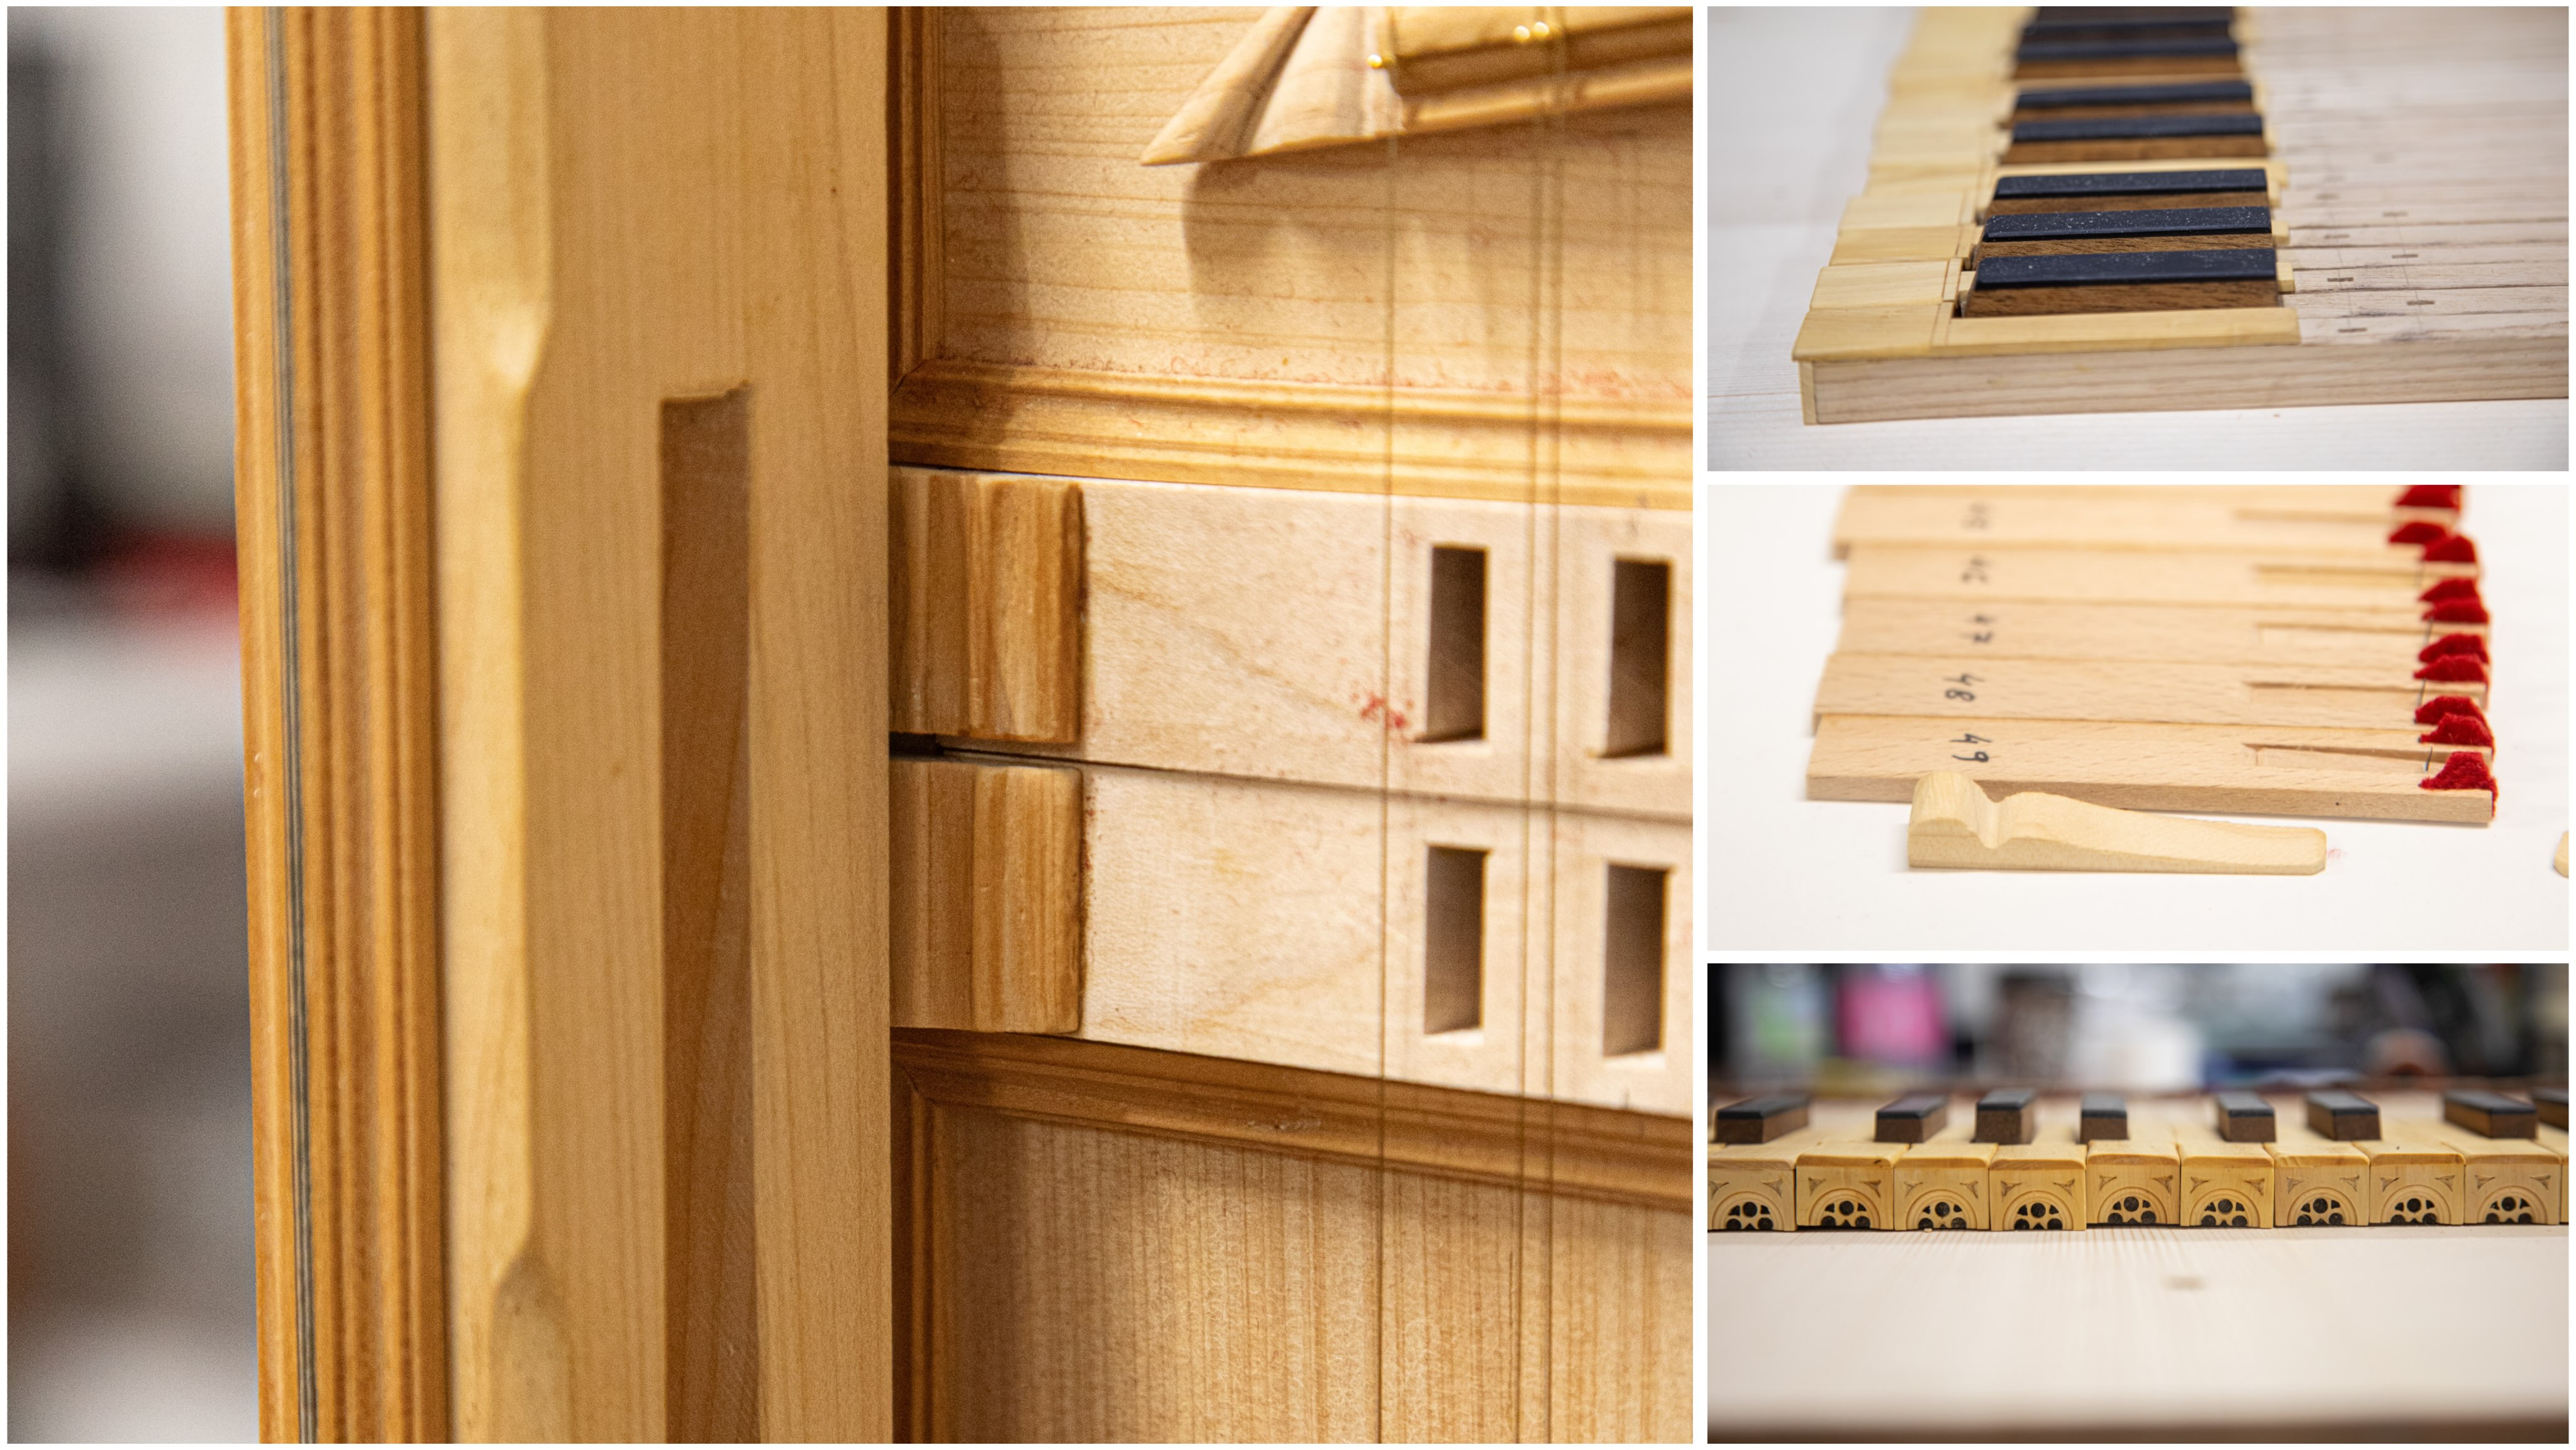
\includegraphics[width=\linewidth]{src/images/details.jpg}
\caption{Details of the replica, including the key slots and sides, keys, and jacks with seagull plectra.}\label{fig:details}
\end{figure*}

The design of the augmented replica keyboard for the Tagliavini Collection was guided by three principal constraints stipulated by the museum:
\begin{itemize}
\item \emph{No visible electronics}. To preserve the visual integrity of the exhibit, all electronic components had to remain concealed except for a pair of headphones and a small display for audio parameter adjustments.
\item \emph{Robustness and reliability}. The system needed to accommodate frequent use by museum visitors and allow for straightforward maintenance by staff without requiring specialised technical expertise.
\item \emph{Faithfulness}. The keyboard mechanism ensured fidelity to its authentic operation, keeping artefacts to a minimum. 
\end{itemize}
These constraints demanded a non-invasive, robust design that was respectful of the historical authenticity of the instruments. The requirement for faithfulness to the original mechanism immediately ruled out a mechanical design reliant on electromechanical actuators, as in previous works on piano haptics \cite{Timmermans2020,Gillespie1996}. While actuators can generate considerable force, they cannot replicate the wideband signals characteristic of the harpsichord's sharp and responsive haptics (A REFERENCE WOULD BE GOOD HERE, ANY IDEAS?), which differ significantly from a piano.



\subsection{Summary of the Finalised Design}

The final design, visible in Figures \ref{fig:teaser} and \ref{fig:details}, is a 49-key harpsichord replica equipped with an optical sensor system reading the amount of light reflected by gradient stickers applied to the jacks' sides. Several key features were implemented to address the project’s requirements:

\begin{itemize}
\item \emph{QRE1113 infrared sensors}. These sensors were selected for their non-invasive properties and precision, enabling the detection of jack displacement without requiring structural modifications to the keyboard mechanism.
\item \emph{Gradient stickers}. Greyscale gradient stickers were applied to each jack to allow the infrared sensors to make precise readings. This approach made calibration easier and enabled scalability from a 3-key prototype to the final 49-key design.
\item \emph{Jack baffles}. Custom-designed baffles, 3D printed from dark pigmented PLA to minimise infrared reflection, were installed around the jacks to prevent cross-talk between adjacent sensors and ensure reliable data capture.
\end{itemize}

\begin{figure}  
  \centering
  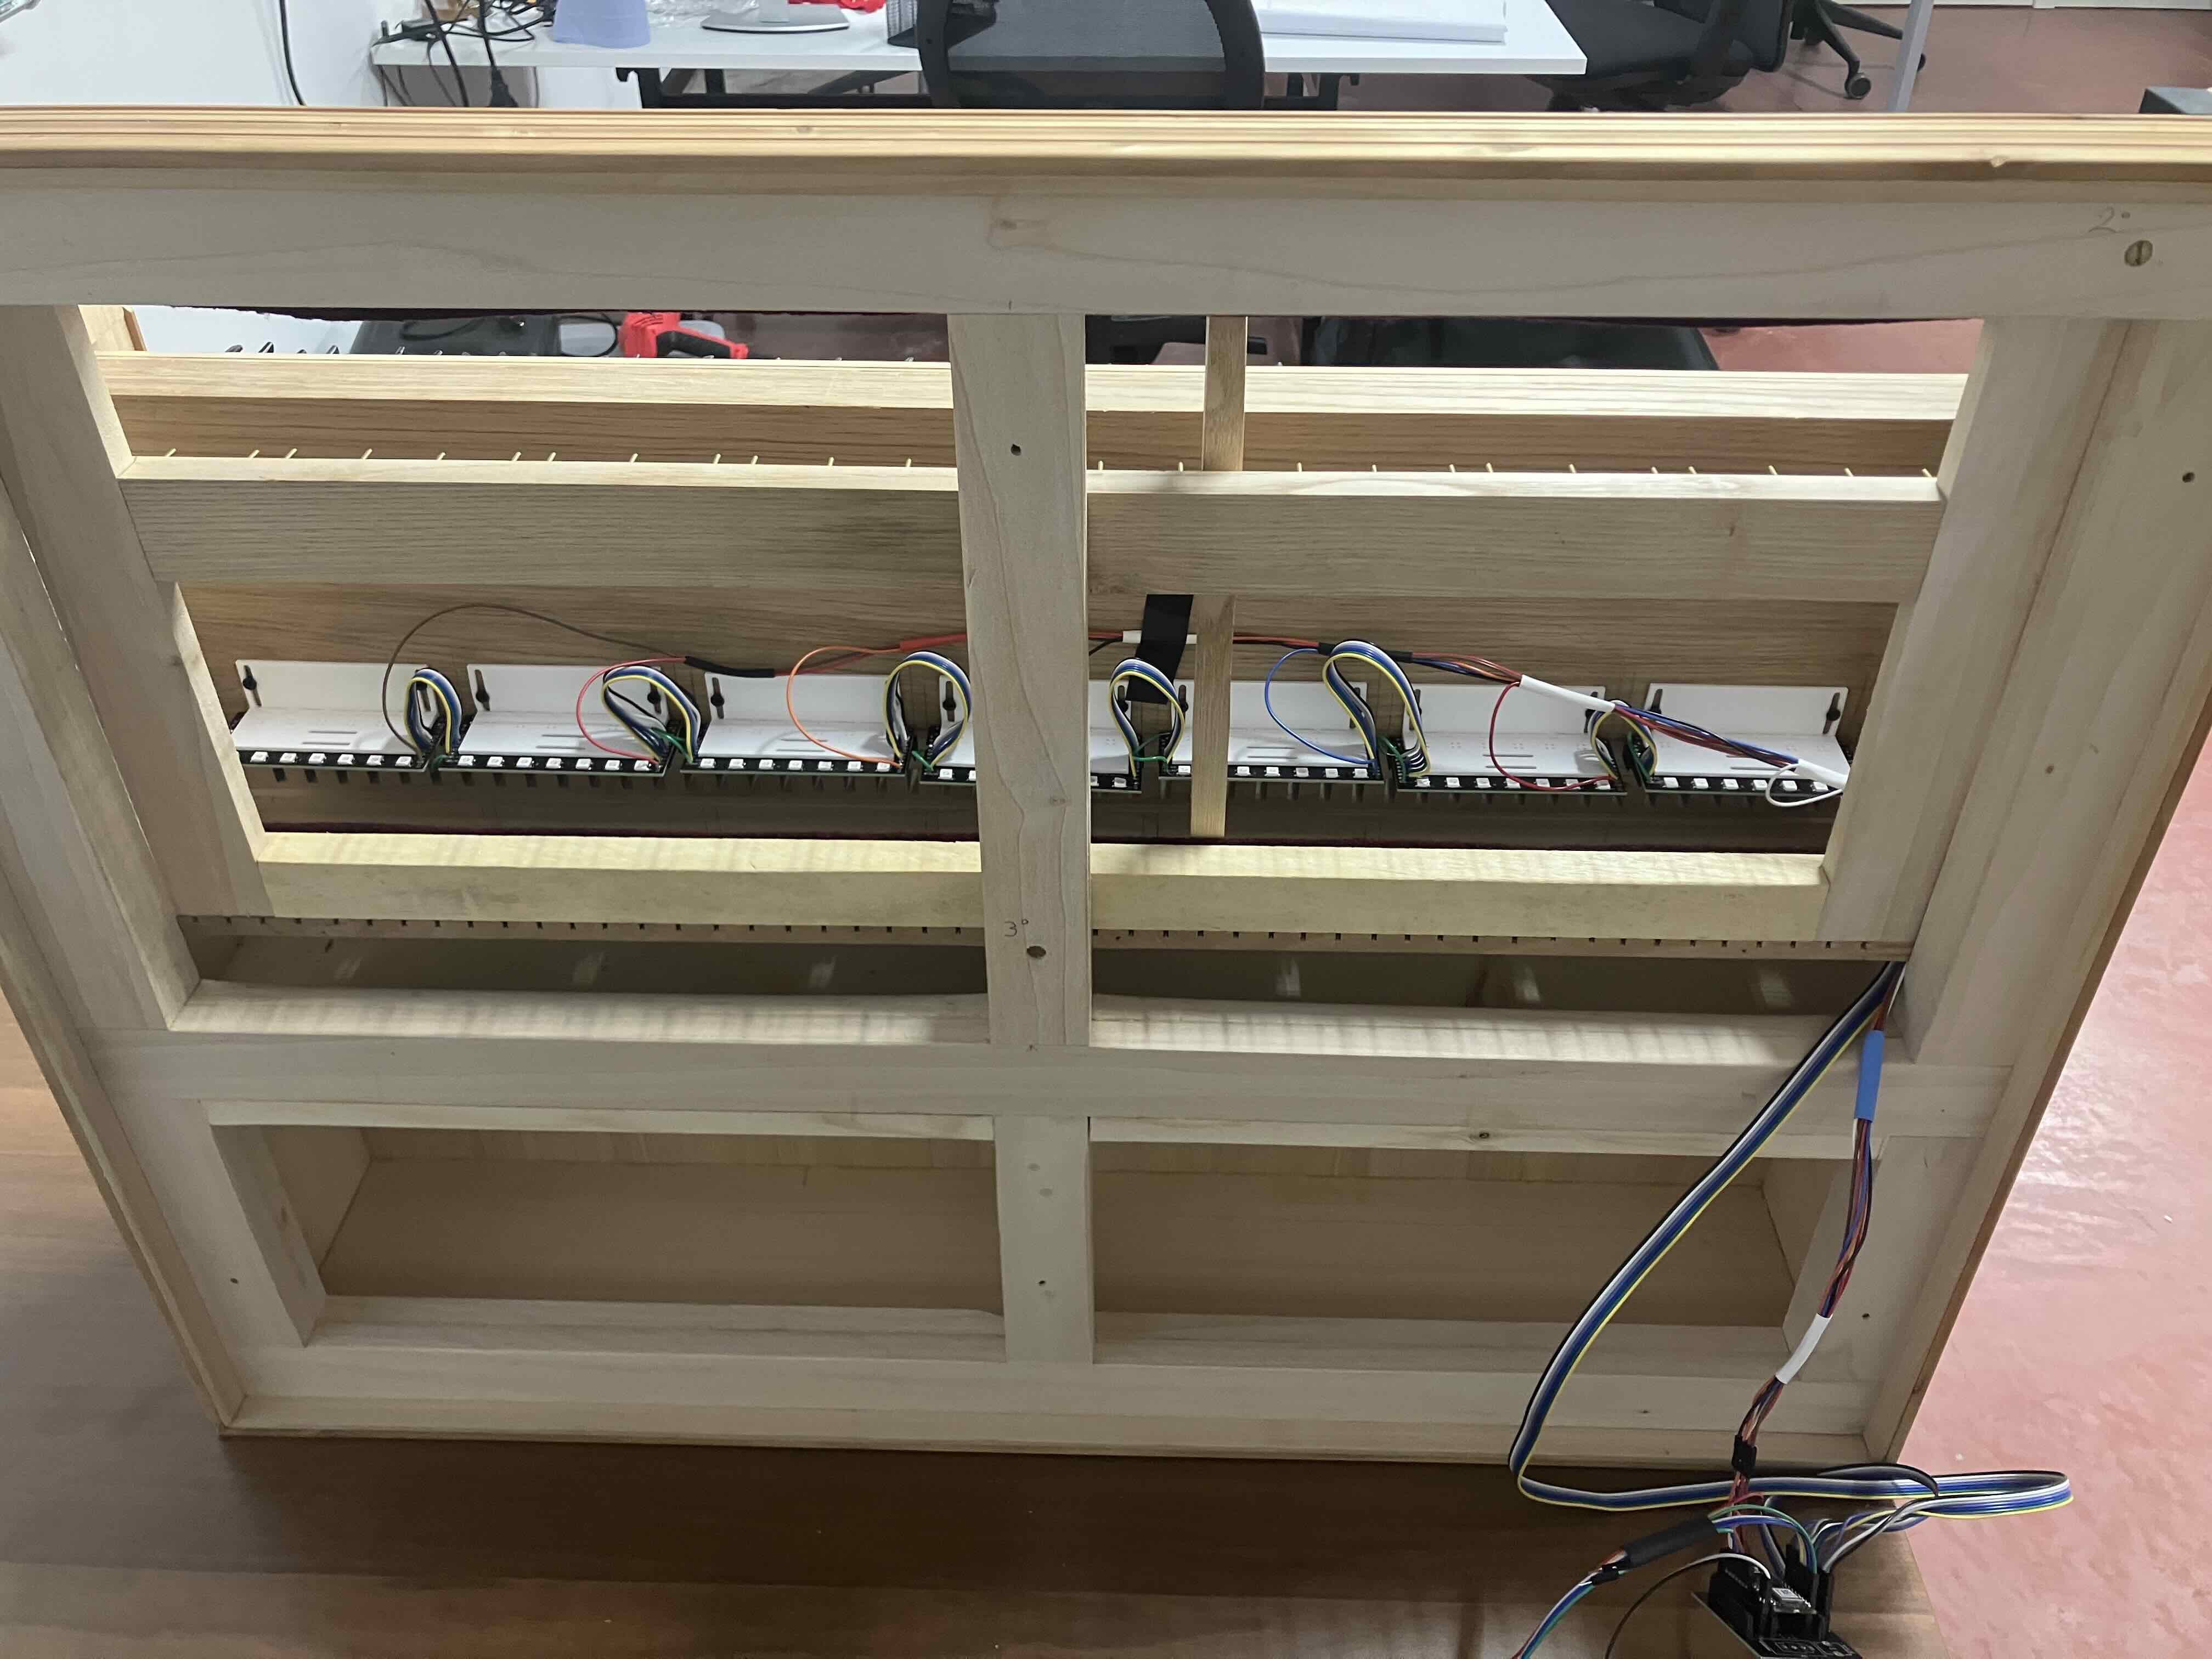
\includegraphics[width=\linewidth]{src/images/49-key-bottom-sensors-no-keys.jpg} 
  \caption{Underside of the full model keyboard, showing two chambers: the front chamber (top) and the rear chamber (bottom).} 
  \Description{} 
  \label{fig:49-key-bottom}
\end{figure}

A modular system of printed circuit boards (PCBs) was designed to manage the sensors and process their output. The 49 QRE1113 sensors were distributed across seven boards, containing 7 sensors each. The PCBs were secured to the underside of the keyboard mechanism, allowing them to be adjusted during installation. Ribbon cables connected the PCBs, providing flexibility during assembly while maintaining a compact form factor. Additional modifications, including baffles and adhesive improvements, were made to optimise the reliability of the sensor system during calibration and use.


The project built upon earlier NIME research on generating MIDI messages from piano keystrokes \cite{McPherson2013}, adapting it to address the unique characteristics of harpsichords and the specified constraints. Whereas the previous design emphasised continuous gesture tracking, this implementation required discrete key-triggered data to align with the needs of MIDI-triggered audio playback. 

\subsection{Project Deployment}
A further objective, set forth by the authors, was to ensure accessibility and reproducibility by committing to an \emph{open-source} approach for all hardware, software, and data. The commitment to open-sourcing encompassed all aspects of the system, including hardware schematics, firmware, and calibration data. Cost-effectiveness was also a central consideration. The system was initially developed for a 3-key prototype, shown in Figure \ref{fig:3key}, and successfully scaled to 49 keys without significant increases in cost or complexity. Specifically, the system was designed to be easily assembled using resources typically available in a university-managed makers space.


Components, such as QRE1113 sensors and CD4051BE multiplexers, are widely available from commercial resellers, while the modular PCB design ensures easy replication and maintenance.

The Arduino Nano BLE was chosen as the core microcontroller for its compatibility with open-source tools and ability to support both USB and BLE MIDI. Ferroelectric RAM (FRAM) was employed for data storage since it offers an economical yet robust solution for preserving calibration settings across power cycles. Calibration workflows were optimised using the Arduino IDE’s serial plotter and open-source MIDI Monitor software, reducing reliance on proprietary tools and simplifying the process for users. 

Reference repositories for this project can be found here. PLEASE FILL OUT AS APPROPRIATE (and anonymise).

\subsection{Materials and Construction}

The keyboard was designed to replicate the tactile and aesthetic sensations of playing an antique Italian harpsichord. Traditional materials were used, including walnut for the wrestplank, chestnut for the key levers, boxwood and ebony for key covers, and cypress for the case and soundboard. The 98 jacks were made from beech, fitted with brass springs and natural seagull feather plectra. The design was inspired by Venetian harpsichords, particularly the Alessandro Trasuntino instrument at the San Colombano Museum. 

The rectangular poplar frame deviates from the traditional logarithmic form to allow for the installation of the electronic sensors, as visible in Figure \ref{fig:49-key-bottom}, without compromising the visual or tactile authenticity. Two string orders, crafted from yellow brass wire and anchored with wrought iron pins, were tensioned to replicate authentic plucking resistance. Felt strips were added to dampen vibrations. The result is an interface that combines the mechanical action of keys with synthetic sound generation, preserving a real harpsichord's tactile and auditory qualities.


\section{Hardware Design}\label{hardware-design}

Figure \ref{fig:system-block-diagram} shows a block diagram of the finalised hardware setup. The system evolved through iterative prototyping, beginning with simple threshold-based testing and ending in a fully functional multi-sensor interface capable of triggering MIDI events. 

\subsection{Prototyping and Key Model}

The initial stage of development focused on testing whether sensor data could reliably trigger MIDI playback. Modifying an existing harpsichord for testing was considered but ultimately discarded due to significant internal measurement and layout discrepancies. Instead, a custom 3-key harpsichord mechanism (Figure \ref{fig:3key}) was acquired from the museum and used as a foundation for prototyping. This approach followed a methodology similar to that used in Timmermans \emph{et al.}'s Haptic Key project \cite{Timmermans2020}, since the 3-key model enabled iterative testing of individual components, including sensor placement, signal processing, and mechanical tolerances, before upscaling. 

\begin{figure}
    \centering
    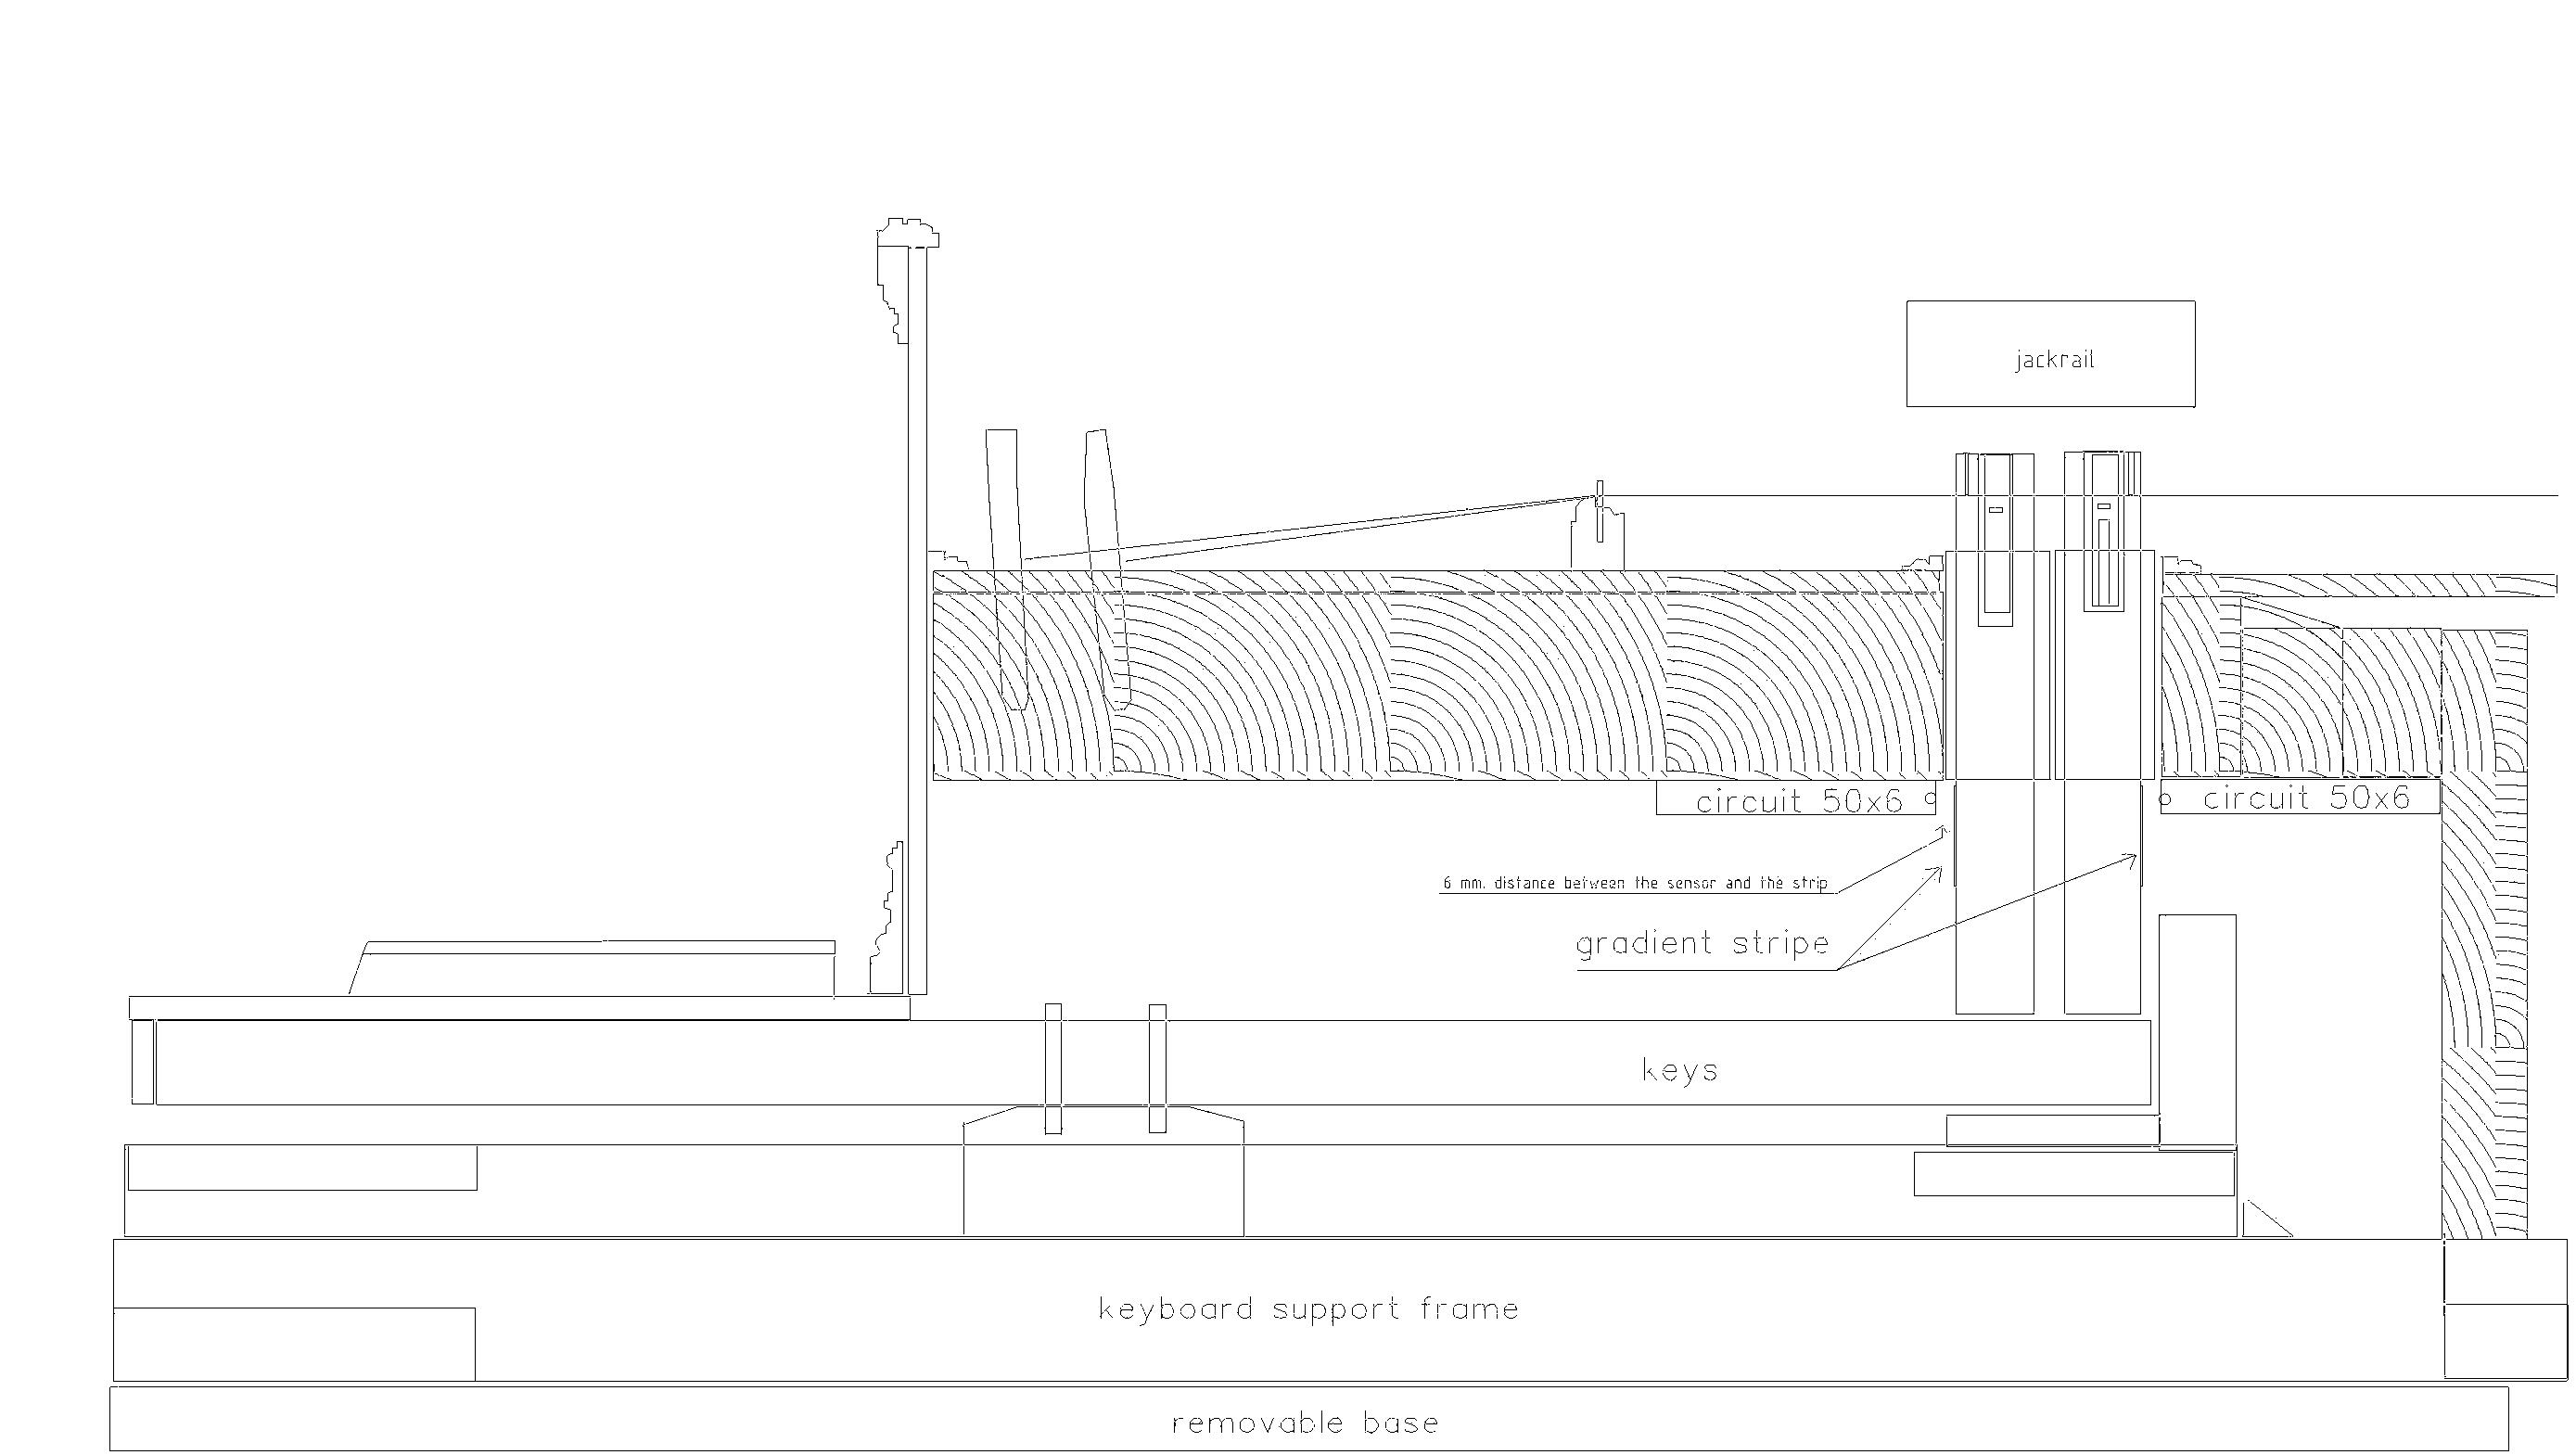
\includegraphics[width=\linewidth]{src/images/CrossSectionSensorPlacement.jpg}
    \\
    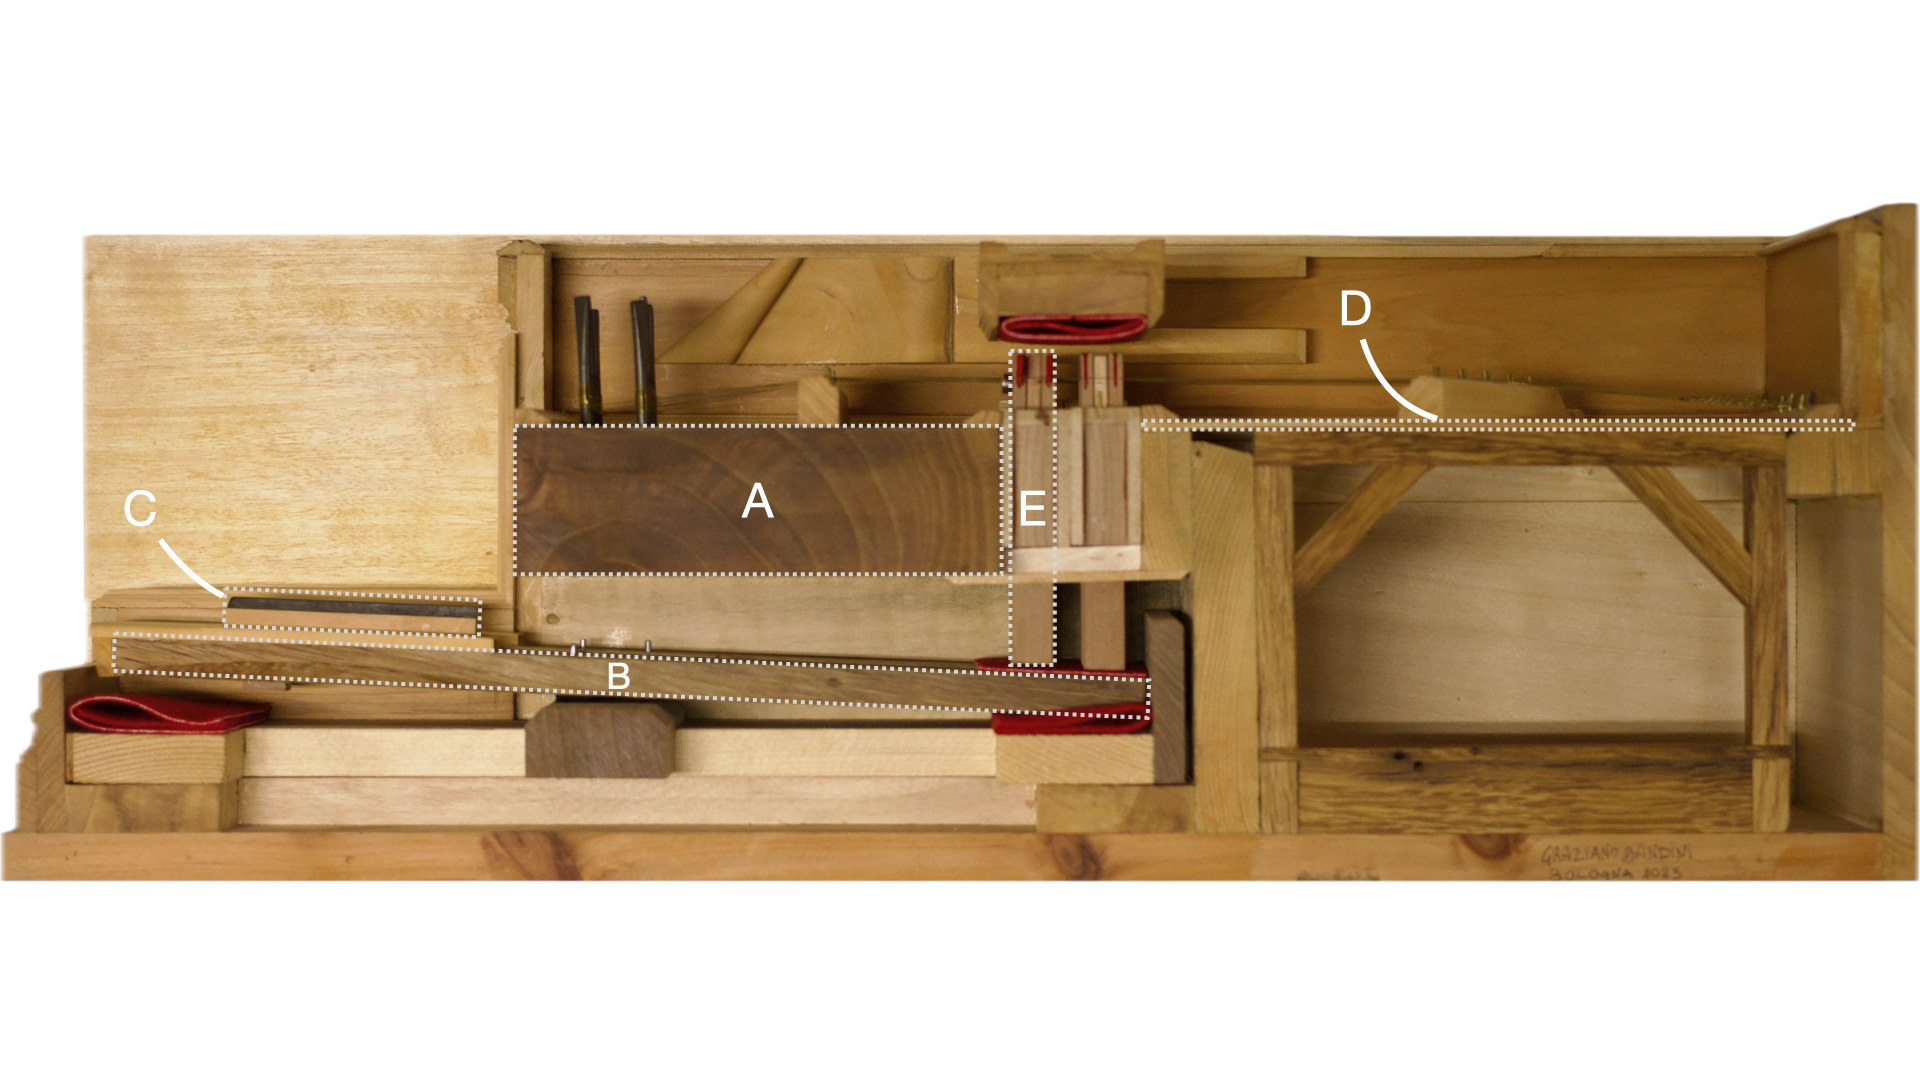
\includegraphics[width=\linewidth]{src/images/3-key-side-labelled.png}
    \caption{3-Key Model Harpsichord Mechanism designed by Graziano Bandini at San Colombano, Bologna, 2023. Key components include A: Wrestplank, B: Key Lever, C: Key Cap, D: Soundboard, E: Jack.}
    \label{fig:3key}
\end{figure}


\subsection{Sensor Criteria}\label{sensor-criteria}

The following criteria were established to guide sensor selection and integration to make the system suitable for a museum context:

\begin{itemize}
    \item \emph{Non-invasiveness.} Sensors must not require significant modifications to the harpsichord's mechanical structure or aesthetics.
    \item \emph{Low Latency.} Sensor response times were required to remain under 10 ms, with an upper limit of 25 ms deemed acceptable, following empirical criteria found in previous studies \cite{Jack2016}.
    \item \emph{Reliability:} Sensor data had to be accurate, minimising false positives and negatives without excessive filtering.
    \item \emph{Scalability.} The design needed to be cost-effective and adaptable for up to 49 keys while maintaining consistent performance.
    \item \emph{Expandability.} The system should accommodate future functionality, such as additional MIDI parameters or data visualisation.
\end{itemize}

The open-source ethos of the project ensured assembly was made possible in standard maker spaces without specialised equipment and provided further guidance in design choices.  

\subsection{Sensor Board Design}\label{sensor-board}

\begin{figure*}
    \centering
    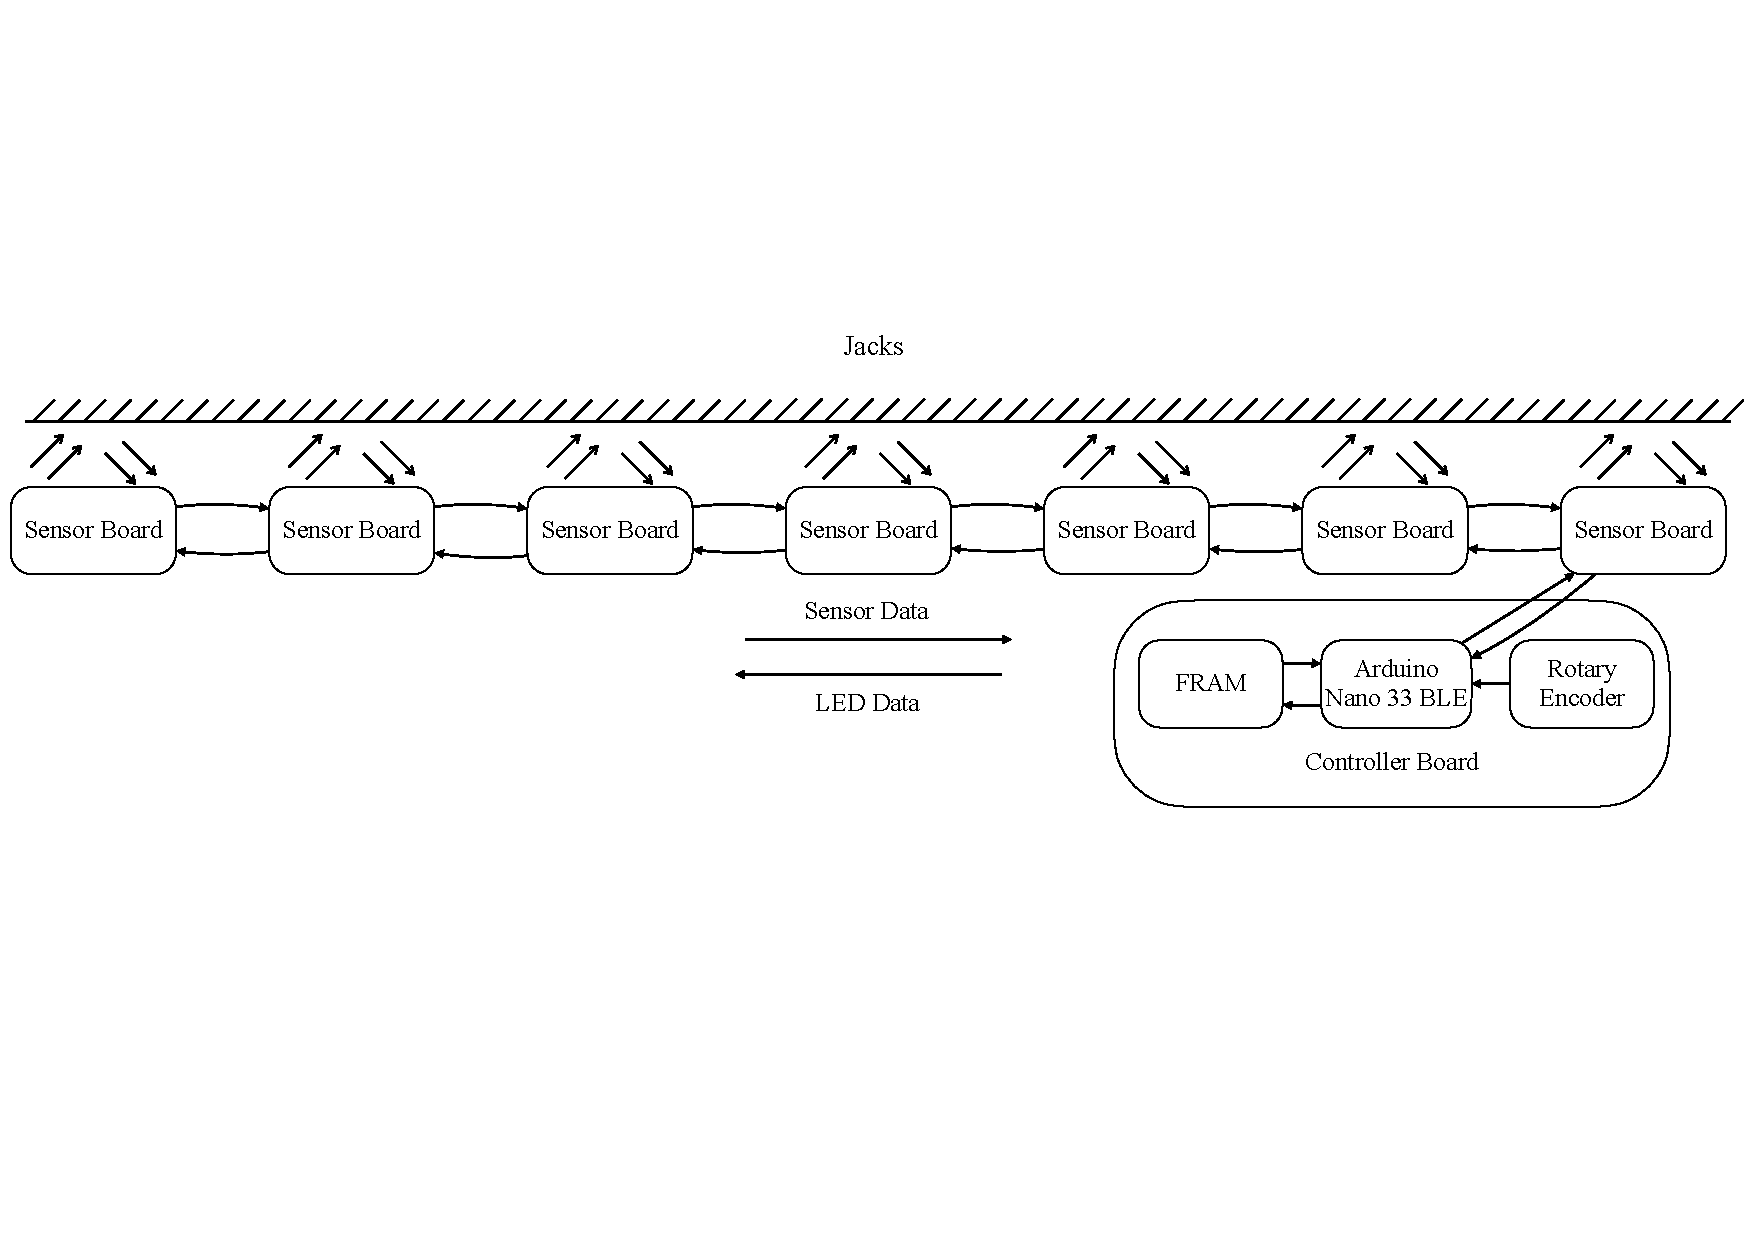
\includegraphics[width=\linewidth]{src/images/block-diagram.pdf}
    \caption{Block diagram of PCB connections. Sensor and LED are routed through each sensor PCB}
    \label{fig:system-block-diagram}
\end{figure*}

The final sensor system utilised QRE1113 infrared sensors, known for their precision and suitability for short-distance detection \cite{McPherson2013, McPherson2019}. The sensors were distributed across seven printed circuit boards (PCBs), each responsible for seven keys. Each PCB contained the following components:

\begin{itemize}
    \item 7 QRE1113 infrared sensors.
    \item 7 100 $\Omega$ resistors and 7 10 k$\Omega$ resistors (later reduced to one resistor per board).
    \item 1 Texas Instruments CD4051BE multiplexer for signal aggregation.
\end{itemize}

The QRE1113 sensors detect infrared light reflected from nearby surfaces, as per the scheme in Figure \ref{fig:simple-schematic}. The gradient stickers affixed to each jack provided a consistent reflective surface for the sensors, which were used to track jack displacement precisely. This easily scalable system allowed straightforward progress from the 3-key prototype to a 49-key model without significant modifications.

\begin{figure}[b]  
  \centering
  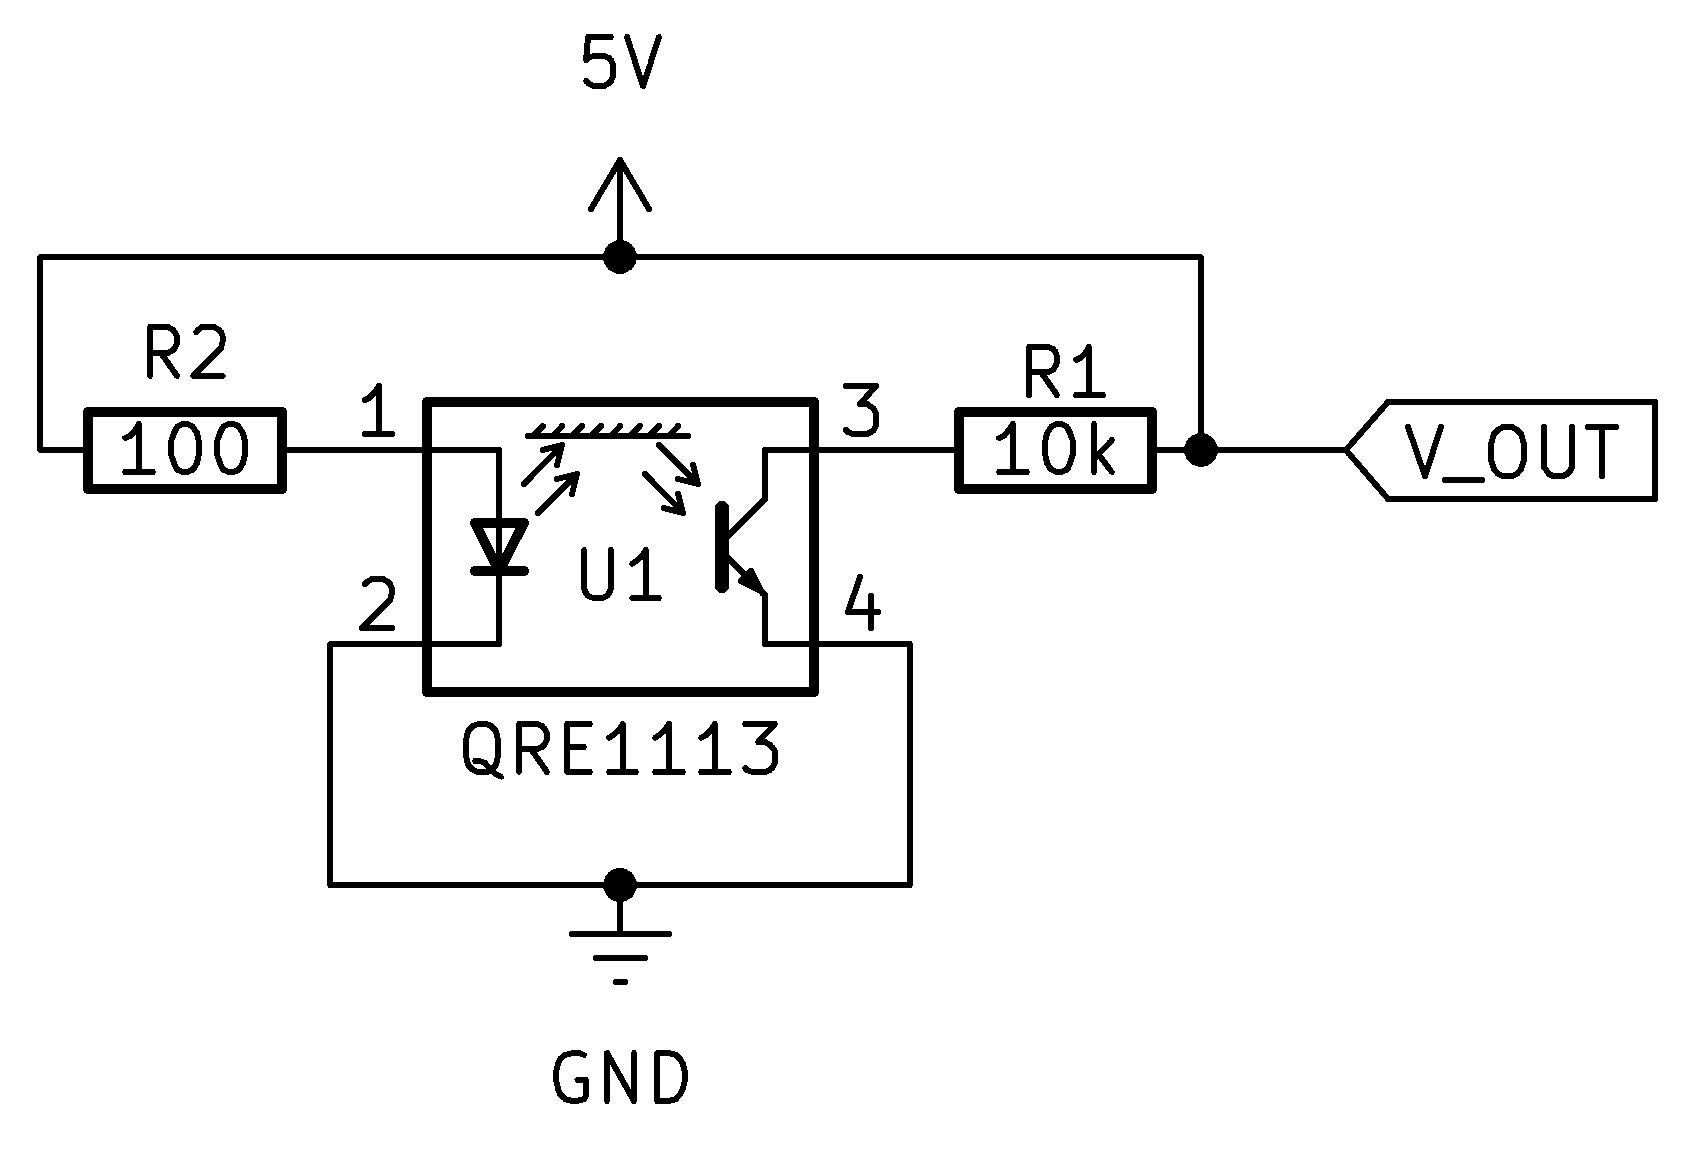
\includegraphics[width=\linewidth]{src/images/simple-schematic-bw-.jpg} 
  \caption{Optical sensor in a simple voltage divider circuit. \texttt{V\_OUT} is routed to one of 8 channels on the CD4051BE multiplexer}
  \Description{} 
  \label{fig:simple-schematic}
\end{figure}



3D-printed baffles were installed on the PCBs to eliminate cross-talk between adjacent sensors, as per Figure \ref{fig:baffles}. These baffles, fabricated from dark-pigmented PLA, ensured that infrared reflections from neighbouring jacks did not interfere with sensor readings. Testing confirmed that this measure significantly improved data reliability.


\begin{figure}
    \centering
    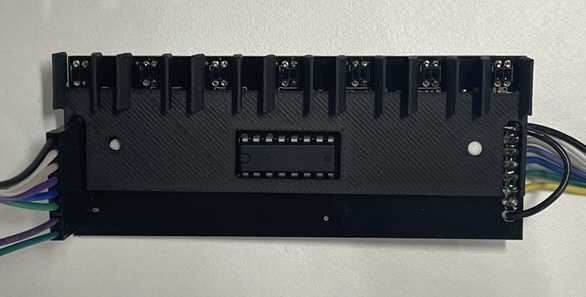
\includegraphics[width=\linewidth]{src/images/sensor-board-w-baffles.jpeg}
    \\
    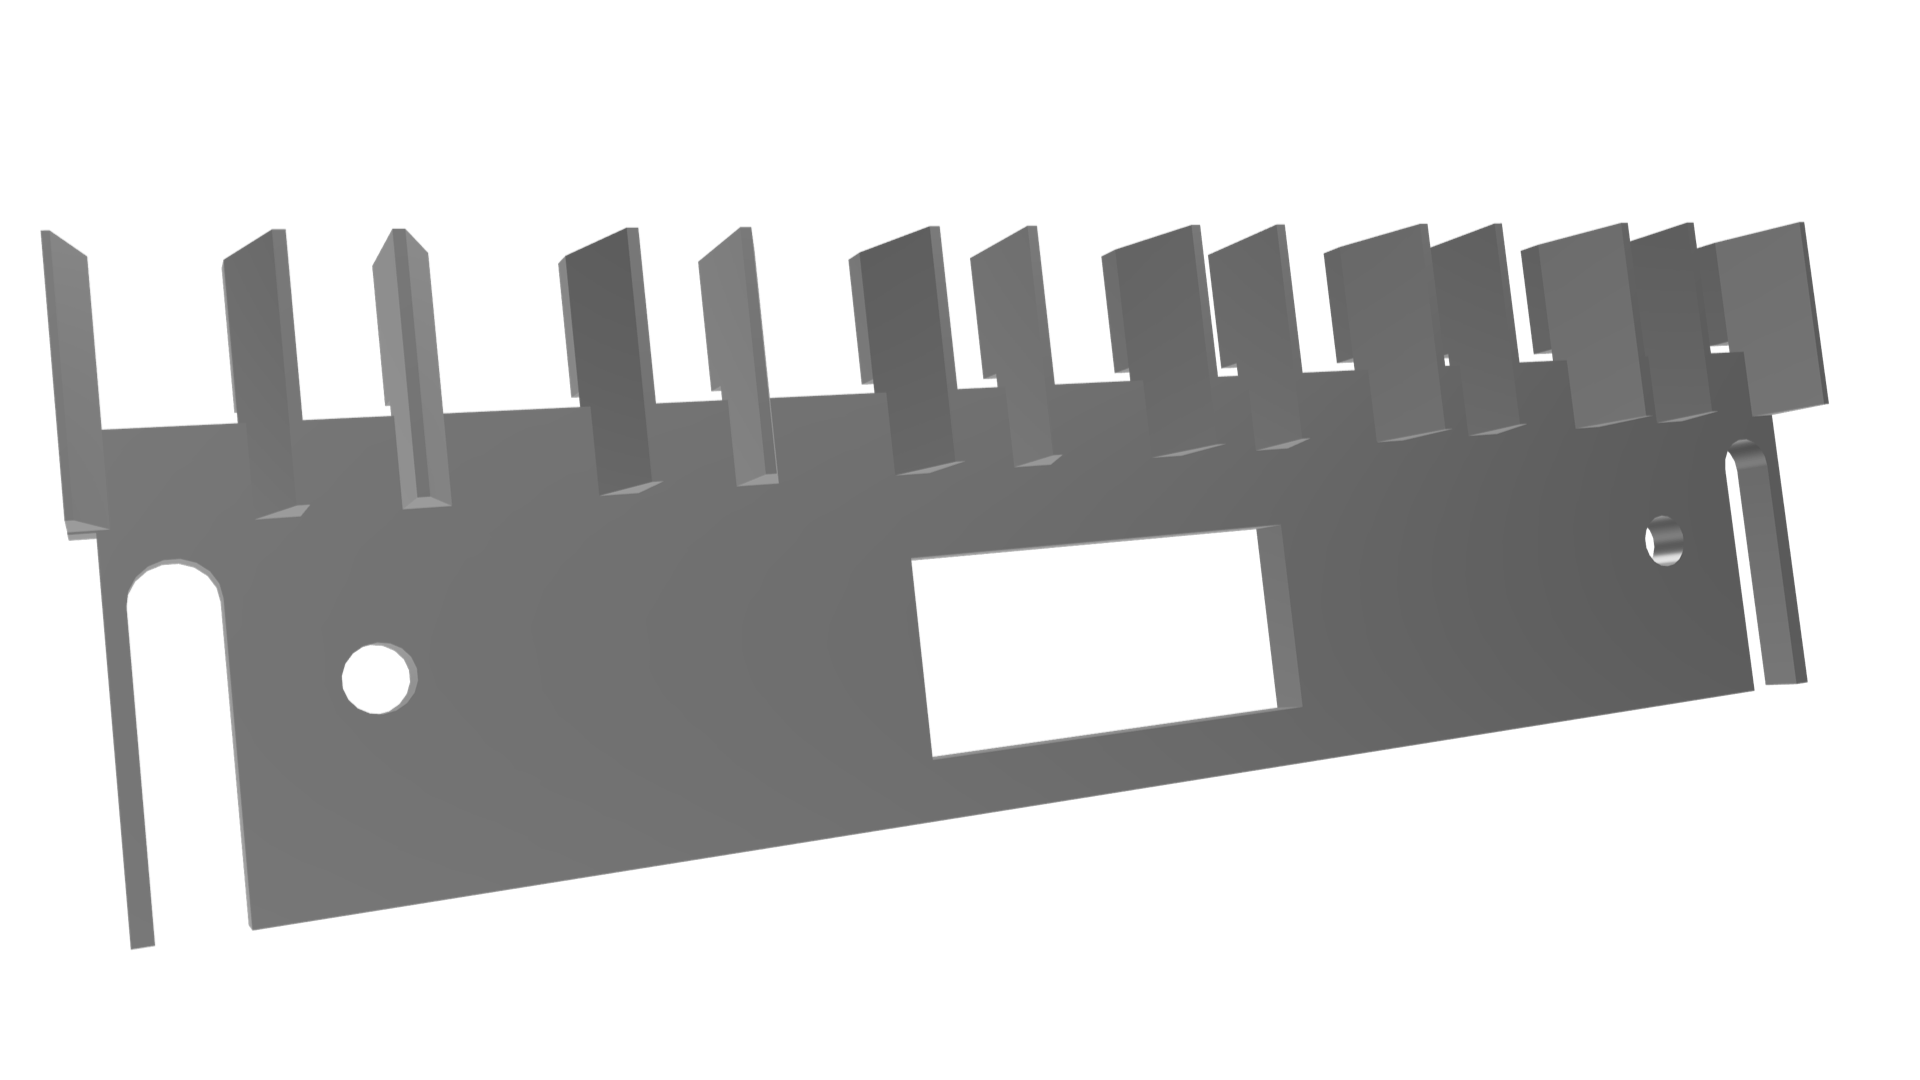
\includegraphics[width=\linewidth]{src/images/baffles.png}
    \caption{Baffles designed to prevent cross-talk between adjacent sensors.}
    \label{fig:baffles}
\end{figure}
\subsection{Controller Board}\label{controller-board}

The controller board, designed around the Arduino Nano BLE platform, was the central hub for processing sensor data and triggering MIDI messages. The Nano BLE was selected for its compact form factor, integrated BLE MIDI functionality, and native USB support. 

Initial iterations used 2.54 mm pitch headers for cable connections, but issues with cable disconnections led to the adoption of JST-PH connectors in later designs. Custom cable looms were constructed using adapted crimping tools, ensuring robust connections without compromising accessibility.

Non-volatile memory, implemented using Ferroelectric RAM (FRAM), provided a reliable means of storing calibration data. This ensured that sensor thresholds and other settings could be preserved across power cycles, enhancing the system's usability in museums.

\subsection{Calibration and Power Management}\label{calibration}

Each sensor's threshold was manually adjusted using RGB LEDs integrated into the system. These LEDs provided visual feedback during calibration, enabling the identification of malfunctioning sensors and simplifying the alignment process. The calibration workflow utilised the Arduino IDE serial plotter and open-source MIDI monitoring software, as per Figure \ref{fig:serial_monitor}. 



As an expert harpsichord performer, finer calibration was carried out with the guidance of \anon{Catalina Vincens}.

Power requirements for the system were estimated at 1.1 A at 5 V, with fluctuations during startup. While the sensors were powered continuously in this iteration, future designs may incorporate power-saving measures, such as dynamic activation of sensors based on usage.


\begin{figure}
    \centering
    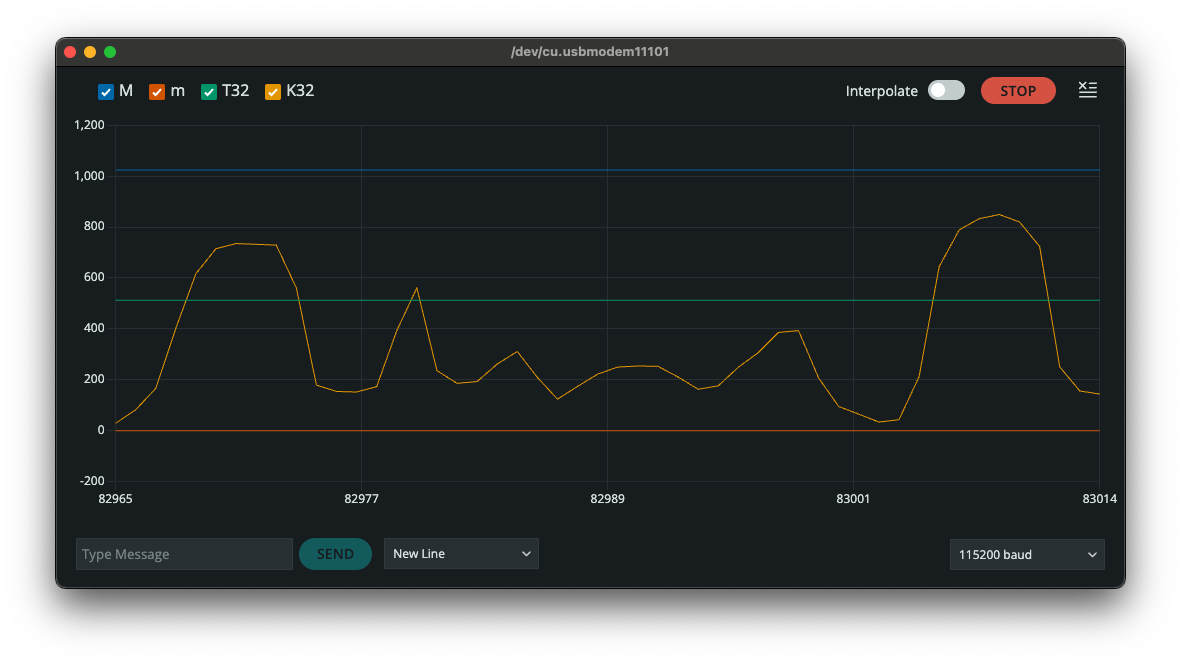
\includegraphics[width=\linewidth]{src/images/serial_monitor.png}
    \caption{Arduino IDE serial plotter used for calibration of sensor thresholds. \texttt{M} and \texttt{m} represent the maximum an minimum value of digitised data. \texttt{K} and \texttt{T} are the values of the sensor and threshold being calibrated, followed by a two-digit number denoting the sensor index (in this case, sensor 32).}
    \label{fig:serial_monitor}
\end{figure}

\subsection{Final Assembly and Integration}

The final 49-key harpsichord replica incorporated the sensor and controller boards into a rectangular frame, deviating slightly from traditional designs to accommodate electronic components. Ribbon cables connected the PCBs, while felt strips were interwoven between the strings to suppress vibrations and maintain the tactile response of the keys.

The assembly process at the NEMUS lab in Bologna involved meticulous adjustments to key clearances and wiring layouts. Modifications included milling sections of the keys to ensure adequate clearance for the PCBs and varnishing the jacks to improve sticker adhesion.

\section{Context}\label{context}

Designed as part of an exhibition for the museum San Colombano in Bologna. Instruments are to be played by the general public to interact with items in the collection that are no longer in playing condition. The audience of one who listens via headphones. The interface strings are damped with felt strips. The damping did change the tension and therefore the feel of the strings so
adjustments needed to be made to the tuning to accomodate for this.

\begin{itemize}
\item
  in museum context
\item
  strings damped
\item
  headphones
\item
  interfacing with kontakt spitfire library
\item
  display

  \begin{itemize}
  \item
    secure storage and access
  \item
    interface to the public
  \end{itemize}
\end{itemize}



\section{Conclusion}\label{conclusion}

Paper has presented the design for an interactive exhibition at a musical instrument museum. Design attempts to address the problem.
Optical sensors read by a microcontroller have been shown to be a solution to tracking vertical displacement of harpsichord jacks and therefore a viable system to augmenting harpsichords. The interface's capabilities of the jack rails to disengage and to convert string plucks to MIDI data means this can be used as a probe to explore how the ``double-pluck'' can be used as vector for expression during performance. The placement of the instrument as a museum exhibit means it also has potential to be used in a long form study.

\section{Going forward}\label{going-forward}

The current interface is an advanced prototype, but there remain many avenues to explore and aspects of the design to improve.

The stickers as a sensor surface have a few limitations that can be addressed. Firstly, the stickers need to be applied manually, which is laborious but also introduces variability. Secondly, the material for the stickers is rated at a 4 years lifespan before the adhesive will decay. The application is non-standard and it is likely there will be failure or drift in sensor readings over time, though to what extent is unknown. This presents a problem on how this approach can be maintained in the long term. Preliminary tests with 3D printed jack bodies incorporating the sensor surface were made. The jack body was notched and effectively acts a shutter against the optical sensor. More testing needs to be carried out before they are incorporated into the design. 3D printed jacks would solve two problems simultaneously in that they would be easily reproducible, but also remove labour demands on the luthier.

Their are also plans to develop the current setup by incorporating force-sensitive resistors (FSR). 
FSRs would be used in conjunction with the current optical sensors to research if an impulse response for the pluck can be extrapolated.


Space constraints meant that only one row of jacks could be sensed. A subsequent redesign in the dimensions of the PCB addressed this problem.
The redesign included flat flex cable (FFC) instead of header pins. This reduced the the size of the PCBs as well as the labour on hand soldering.
There was an additional added benefit in that the FFC has only a single orientation in which it conducts, meaning it cannot be incorrectly connected.

Currently the instrument communicates with a Spitfire sample library through the Kontakt software sampler. As such, the full data from both rows of jacks cannot be utilised. which is limited. A future output of the \anon{NEMUS} project will be a bespoke sound synthesis engine to leverage data from both jack rows
which will also be open-sourced. The intention is also to create a numerically simulated non-linear plucked string models with which the device can interact. 


A second interface designed more closely to the Trasuntino style instrument has been commissioned by the \anon{NEMUS} project with \anon{Roberto Livi}. 
Using lessons learned for the first iteration the second can make better accommodations for internal electronics. Interface to be used for a performer study and used for performance with the aforementioned numerically simulated sound synthesis engine.

Future novel designs for an interface that would utilise available data, such as velocity and aftertouch, in software in the manner of a hyperinstrument.
Currently the system looks for the cross over a threshold for triggering MIDI messages, but jack displacement is tracked continuously. Data for velocity, both of the pluck and the jack can be extracted from the available data, simply requiring the addition of state machine to make use of it.

Seat vibrations \cite{MusicalHaptics2018_07} can also be explored to determine if they would create a more immersive experience in the exhibition context.



A current limitation is the latency in triggering MIDI output. Currently the latency from pressing a key to triggering a note is around 20 ms. 
The latency should ideally be closer to 10 ms and with no jitter so \cite{Jack2016}.

One approach would be to change the microcontroller. A test
was carried out using an Arduino Nano ESP32 which is a NORA-W106, a module containing an ESP32-S3. 
The benefit of this microcontroller is that it would allow the microcontroller to be swapped and the rest of the PCB
designs would be unaffected.

Another approach would be to use a different microcontroller entirely. 
Some research was carried during the course of the project using an ESP32 programmed with the Espressif development framework ESP-IDF. 
The same logic as the original firmware was programmed and the latency was reduced to below 10 ms. ESP-IDF allows access to functionality of the ESP32 including regular processing of an internal audio buffer that is not exposed in the Arduino IDE. 
It is possible that the 10 ms latency could be improved upon with appropriate optimisation, but there would be a cost in the form of development time. 
Consideration would need to be made on the time to port existing source code for the I2C FRAM chip or fall back on a simpler storage option.


\section{Ethical Standards}\label{ethical-standards}

To ensure objectivity and transparency in research and to ensure that
accepted principles of ethical and professional conduct have been
followed, authors must include a section ``Ethical Standards'' before
the References. This section should include (if relevant): information
regarding sources of funding, potential conflicts of interest (financial
or non-financial), informed consent if the research involved human
participants, statement on welfare of animals if the research involved
animals or any other information or context that helps ethically situate
your research. For help with the ethics section, feel free to ask on the
NIME forum: \url{https://forum.nime.org}.


% \begin{tikzpicture}[auto, node distance=2cm,>=latex']

%     \node [input, name=input] {};
%     \node [sum, right of=input] (sum) {};
%     \node [block, right of=sum] (controller) {Controller};
%     \node [block, right of=controller, pin={[pinstyle]above:D},
%             node distance=3cm] (system) {System};

%     \draw [->] (controller) -- node[name=u] {$u$} (system);
%     \node [output, right of=system] (output) {};
%     \node [block, below of=u] (measurements) {Measurements};

%     \draw [draw,->] (input) -- node {$r$} (sum);
%     \draw [->] (sum) -- node {$e$} (controller);
%     \draw [->] (system) -- node [name=y] {$y$}(output);
%     \draw [->] (y) |- (measurements);
%     \draw [->] (measurements) -| node[pos=0.99] {$-$} 
%         node [near end] {$y_m$} (sum);
% \end{tikzpicture}